%TODO: provide your details here.



\begin{frame}
    \frametitle{About Your Fellows}
    \begin{itemize}
        \item Hi there! We are \textcolor{red}{\textbf{Hamza}} {and }\textcolor{red}{\textbf{Umer}}.
        \item We are Associate Students at ITU.
    \end{itemize}
\end{frame}



\begin{frame}{Topological Sorting Algorithm}
    \textbf{Step 1:} Given a Directed Acyclic Graph (DAG) \( G = (V, E) \). \\
    \textbf{Step 2:} Compute the in-degree \( d(v) \) for each vertex \( v \in V \). \\
    \textbf{Step 3:} Initialize an empty list \( \text{topological\_order} \) and a queue \( W \). \\
    \textbf{Step 4:} Add all vertices \( v \) with \( d(v) = 0 \) to \( W \). \\
    \textbf{Step 5:} While \( W \) is not empty, repeat the following: \\
    \hspace{1cm} a) Remove a vertex \( u \) from \( W \). \\
    \hspace{1cm} b) Append \( u \) to \( \text{topological\_order} \). \\
    \hspace{1cm} c) For each vertex \( v \) such that \( (u, v) \in E \): \\
    \hspace{2cm} i) Remove edge \( (u, v) \). \\
    \hspace{2cm} ii) Decrease in-degree \( d(v) \) by 1. \\
    \hspace{2cm} iii) If \( d(v) = 0 \), append \( v \) to \( W \). \\
    \textbf{Step 6:} The list \( \text{topological\_order} \) contains the topological ordering of the graph. \\
\end{frame}





\begin{frame}{Example: Step 1 - Initial Graph}
\textbf{Solving an Example:} 
Let's apply the topological sorting algorithm to this Directed Acyclic Graph.

\vspace{0.3cm} % Increase space before the graph
\centering
\begin{tikzpicture}
    % Positioning Nodes with More Space
    \node (a) [circle, draw] {a};
    \node (b) [circle, draw, right=2cm of a] {b};
    \node (c) [circle, draw, below=2cm of b] {c};
    \node (d) [circle, draw, right=2cm of b] {d};
    \node (f) [circle, draw, below=2cm of d] {f};
    \node (e) [circle, draw, right=2cm of d] {e};

    % Adjusted Arrows with Bending
    \draw[->] (a) -- (b);
    \draw[->] (a) -- (c);
    \draw[->] (b) -- (d);
    \draw[->] (c) edge[bend left] (f); % Avoids overlap
    \draw[->] (d) -- (e);
    \draw[->] (d) edge[bend right] (f); % Avoids overlap
\end{tikzpicture}

\vspace{0.3cm} % Adds more space between graph and explanation
\textbf{Explanation:} This is the given directed acyclic graph (DAG). The goal is to perform topological sorting by iteratively removing nodes with an in-degree of 0.
\end{frame}


\begin{frame}{Step 2: Remove $a$ (in-degree 0)}
\centering
\begin{tikzpicture}
    \node (b) [circle, draw] {b};
    \node (c) [circle, draw, below=1cm of b] {c};
    \node (d) [circle, draw, right=1.5cm of b] {d};
    \node (f) [circle, draw, below=1cm of d] {f};
    \node (e) [circle, draw, right=1.5cm of d] {e};

    \draw[->] (b) -- (d);
    \draw[->] (c) -- (f);
    \draw[->] (d) -- (e);
    \draw[->] (d) -- (f);
\end{tikzpicture}

\vspace{0.5cm}
\textbf{Explanation:} Node $a$ had no incoming edges (in-degree 0), so we removed it. The edges coming out of $a$ are also removed.
\end{frame}

\begin{frame}{Step 3: Remove $b$, $c$ (in-degree 0)}
\centering
\begin{tikzpicture}
    \node (d) [circle, draw] {d};
    \node (f) [circle, draw, below=1cm of d] {f};
    \node (e) [circle, draw, right=1.5cm of d] {e};

    \draw[->] (d) -- (e);
    \draw[->] (d) -- (f);
\end{tikzpicture}

\vspace{0.5cm}
\textbf{Explanation:} Nodes $b$ and $c$ now have an in-degree of 0 and are removed. Their outgoing edges are also removed.
\end{frame}

\begin{frame}{Step 4: Remove $d$ (in-degree 0)}
\centering
\begin{tikzpicture}
    \node (e) [circle, draw] {e};
    \node (f) [circle, draw, below=1cm of e] {f};
\end{tikzpicture}

\vspace{0.5cm}
\textbf{Explanation:} Node $d$ is now free of incoming edges, so it is removed, along with its outgoing edges.
\end{frame}

\begin{frame}{Final Topological Orders}
\centering
\textbf{Two Valid Topological Orders:}

\vspace{0.5cm}

\textbf{Order 1:} $a, b, c, d, e, f$

\textbf{Order 2:} $a, c, b, d, f, e$

\vspace{0.5cm}

\textbf{Explanation:}
\begin{itemize}
    \item Both orders start with $a$ since it has no incoming edges.
    \item After removing $a$, either $b$ or $c$ can be chosen first.
    \item The rest of the ordering follows the dependency constraints of the DAG.
\end{itemize}

\vspace{0.5cm}
\textbf{Conclusion:} There can be multiple valid topological sorts in a DAG as long as dependencies are maintained.
\end{frame}




\begin{frame}{Minimum Spanning Tree (MST)}
\textbf{Definition:}  
A \textbf{Minimum Spanning Tree (MST)} is a subset of the edges in a connected, weighted graph that:
\begin{itemize}
    \item \textbf{Spans the entire graph:} It includes all the vertices of the original graph.
    \item \textbf{Ensures connectivity:} The MST forms a connected subgraph, meaning there are no isolated vertices.
    \item \textbf{Minimizes the total edge cost:} Among all spanning trees, the MST has the smallest possible sum of edge weights.
    \item \textbf{Avoids cycles:} Since it is a tree, it does not contain cycles.
\end{itemize}

\textbf{Key Properties:}
\begin{itemize}
    \item If a graph has \( V \) vertices, the MST will have exactly \( V-1 \) edges.
    \item There can be multiple valid MSTs for a graph.
    \item MSTs are commonly found using algorithms like \textbf{Kruskal's} and \textbf{Prim's}.
\end{itemize}
\end{frame}






\begin{frame}{Cities Graph}
    
\begin{center}
\begin{tikzpicture}[
    scale=0.5, % Reduce overall size further
    every node/.style={scale=0.8}, % Adjust node text size
    roundnode/.style={circle, draw=black, thick, minimum size=0.8cm},
    edge/.style={draw=black, thick}
]

% Nodes (Adjusted for better spacing)
\node[roundnode] (HEL) {HEL};
\node[roundnode, right=1.5cm of HEL] (STP) {STP};
\node[roundnode, below=1.3cm of HEL] (FRA) {FRA};
\node[roundnode, right=1.5cm of FRA] (BER) {BER};
\node[roundnode, right=1.5cm of BER] (WAR) {WAR};
\node[roundnode, below=1.5cm of WAR] (KIE) {KIE};
\node[roundnode, right=1.5cm of WAR] (MOS) {MOS};
\node[roundnode, left=1.5cm of FRA] (MUN) {MUN};
\node[roundnode, below=1.5cm of MUN] (BUD) {BUD};

% Edges (Adjusted to remove overlaps and reduce distances)
\draw[edge] (HEL) -- node[above] {\small 3} (STP);
\draw[edge] (HEL) -- node[left] {\small 5} (FRA);
\draw[edge] (FRA) -- node[above] {\small 12} (BER);
\draw[edge] (BER) -- node[above] {\small 10} (WAR);
\draw[edge] (FRA) -- node[left] {\small 1} (MUN);
\draw[edge] (MUN) -- node[left] {\small 92} (BUD);
\draw[edge] (BUD) -- node[below] {\small 33} (KIE);
\draw[edge] (WAR) -- node[right] {\small 19} (STP);
\draw[edge] (WAR) -- node[right] {\small 27} (MOS);
\draw[edge] (MOS) -- node[right] {\small 35} (KIE);
\draw[edge] (MUN) to[out=-30, in=-150, looseness=1.2] node[below] {\small 6} (BER); % Curved edge below

\end{tikzpicture}
\end{center}

\vspace{0.3cm} % Space before text

\begin{itemize}
    \item Cities are connected through roads.
    \item There is a cost in kilometers between the edges, representing their distance.
\end{itemize}

\end{frame}




\begin{frame}{Introduction to Union-Find}
    \begin{itemize}
        \item Union-Find (Disjoint Set) is a data structure that helps in managing a partition of elements into disjoint sets.
        \item Supports two main operations:
        \begin{itemize}
            \item \textbf{Find}: Determine which set an element belongs to.
            \item \textbf{Union}: Merge two sets.
        \end{itemize}
        \item Used in Kruskal's algorithm, network connectivity problems, etc.
    \end{itemize}
\end{frame}

\begin{frame}{Set Representation (Tree Structure)}
    \begin{itemize}
        \item \textbf{Example:} Two sets represented as trees:
        \item \textbf{Parent nodes} point to their children.
    \end{itemize}

    \centering
    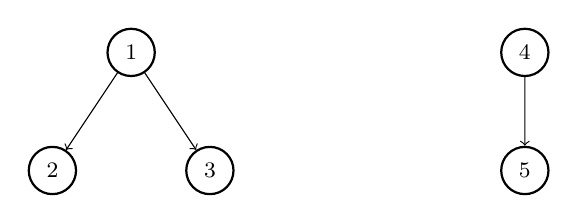
\begin{tikzpicture}[
        every node/.style={draw, circle, minimum size=0.6cm, font=\footnotesize, thick}, 
        level distance=1.5cm, % Increases the distance between levels
        sibling distance=2cm, % Increases the distance between siblings
        every path/.style={thin, ->} % Makes the tree lines thinner
    ]

        % First tree (Set {1,2,3})
        \node (1) {1}
            child {node {2}}
            child {node {3}};

        % Second tree (Set {4,5})
        \node (4) at (5,0) {4}
            child {node {5}};

    \end{tikzpicture}

\end{frame}



\begin{frame}{Find Algorithm}
    \begin{itemize}
        \item The Find(a) function determines the representative (root) of the set containing element a.
        \item If a is not the root, we recursively call Find(π(a)).
        \item Using rank helps keep the tree balanced.
    \end{itemize}

    \vspace{0.5cm}
    \textbf{Pseudocode:}
    \begin{itemize}
        \item \textbf{Find(a):}
        \begin{enumerate}
            \item If \( \pi(a) == a \), return a.
            \item Else, recursively call Find(\(\pi(a)\)).
            
        \end{enumerate}
    \end{itemize}

    \vspace{0.3cm}
    \centering
    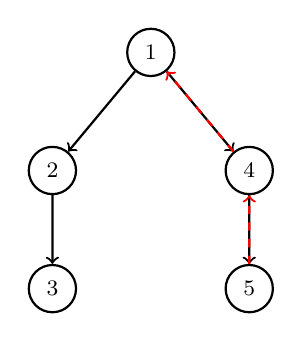
\begin{tikzpicture}[
        every node/.style={draw, circle, minimum size=0.6cm, font=\footnotesize}, 
        level distance=1.5cm, sibling distance=2.5cm,
        every path/.style={thick, ->}
    ]

        % Tree structure
        \node (1) {1}
            child {node (2) {2}
                child {node (3) {3}}
            }
            child {node (4) {4}
                child {node (5) {5}}
            };

        % Highlighted path for Find(5)
        \draw[red, thick, dashed] (5) -- (4);
        \draw[red, thick, dashed] (4) -- (1);
        
    \end{tikzpicture}

    \vspace{0.3cm}
    \textbf{Example:} \textcolor{red}{Find(5) → 4 → 1 (Root)}

\end{frame}



\begin{frame}{Union by Rank}
    \begin{itemize}
        \item We use rank to keep the tree balanced.
        \item The node with the highest rank becomes the parent.
    \end{itemize}

    \begin{center}
        \begin{minipage}{0.5\textwidth}
            \centering
            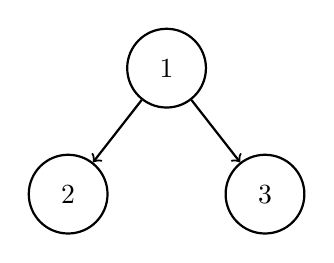
\begin{tikzpicture}[
                every node/.style={draw, circle, minimum size=1cm, font=\normalsize}, 
                level distance=1.6cm, sibling distance=2.5cm,
                every path/.style={thick, ->}
            ]
                % Tree Structure
                \node (1) {1}
                    child {node (2) {2}}
                    child {node (3) {3}};
            \end{tikzpicture}
        \end{minipage}
        \hfill
        \begin{minipage}{0.4\textwidth}
            \textbf{Root Node:} \\
            Parent = 1, Rank = 1

            \vspace{0.5cm}

            \textbf{Left Child (2):} \\
            Parent = 1, Rank = 0

            \vspace{0.5cm}

            \textbf{Right Child (3):} \\
            Parent = 1, Rank = 0
        \end{minipage}
    \end{center}

\end{frame}




% ------------------- Slide 1: Introduction -------------------
\begin{frame}{Union-Find Data Structure}
    \begin{itemize}
        \item A \textbf{Union-Find} (Disjoint Set) data structure helps efficiently manage dynamic connectivity.
        \item Supports two main operations:
        \begin{itemize}
            \item \textbf{Find(x)}: Finds the representative (root) of the set containing `x`.
            \item \textbf{Union(a, b)}: Merges the sets containing `a` and `b` based on \textbf{rank}.
        \end{itemize}
        \item Uses \textbf{Union by Rank} and \textbf{Path Compression} for efficiency.
    \end{itemize}
\end{frame}

% ------------------- Slide 2: Union by Rank -------------------
\begin{frame}{Union by Rank}
    \textbf{Algorithm:}
    \begin{itemize}
        \item Find the parents of `a` and `b`:  
            \[
            x = \text{find}(a), \quad y = \text{find}(b)
            \]
        \item Compare their ranks:
            \begin{itemize}
                \item If \textbf{rank(x) > rank(y)}, set \textbf{parent(y) = x}
                \item If \textbf{rank(y) > rank(x)}, set \textbf{parent(x) = y}
                \item If \textbf{rank(x) == rank(y)}, set \textbf{parent(x) = y} and increment \textbf{rank(y)++}
            \end{itemize}
    \end{itemize}
\end{frame}

% ------------------- Merged Slide: Before and After Union -------------------
\begin{frame}{Example: Before and After Union(2,4)}
    \centering
    \begin{minipage}{0.45\linewidth}
        \centering
        \textbf{\Large Before Union} % Increased size
        \begin{tikzpicture}[
            every node/.style={draw, circle, minimum size=1cm, font=\normalsize}, 
            level distance=1.4cm, sibling distance=1.8cm,
            every path/.style={thick, ->}
        ]
            % Tree 1: Modified layout
            \node (1) {1}
                child {node (2) {2} 
                    child {node (3) {3}}
                };
            
            % Tree 2: Moved closer for better alignment
            \node[right=2.5cm of 1] (4) {4}; 
        \end{tikzpicture}
    \end{minipage}
    \hspace{0.8cm}
    \begin{minipage}{0.45\linewidth}
        \centering
        \textbf{\Large After Union(2,4)} % Increased size
        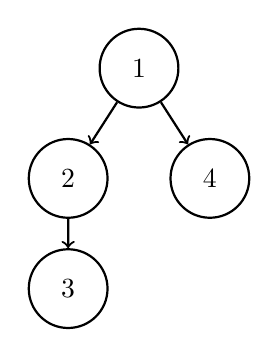
\begin{tikzpicture}[
            every node/.style={draw, circle, minimum size=1cm, font=\normalsize}, 
            level distance=1.4cm, sibling distance=1.8cm,
            every path/.style={thick, ->}
        ]
            % Modified layout for balance
            \node (1) {1}
                child {node (2) {2} 
                    child {node (3) {3}}
                }
                child {node (4) {4}};
        \end{tikzpicture}
    \end{minipage}
\end{frame}


% ------------------- Merged Slide: Path Compression -------------------
\begin{frame}{Path Compression}
    \begin{itemize}
        \item After applying Union, we can optimize \textbf{find(x)} using \textbf{Path Compression}.
        \item Instead of traversing the tree every time, we directly point all nodes to the root.
        \item This reduces the time complexity to \textbf{nearly O(1)} for each operation.
    \end{itemize}

    \vspace{0.5cm}
    \centering
    \begin{tikzpicture}[
        every node/.style={draw, circle, minimum size=1cm, font=\normalsize}, 
        level distance=1.6cm, sibling distance=1.8cm,
        every path/.style={thick, ->}
    ]
        % Before Path Compression (Shifted Left)
        \node at (-2,0) (1) {1}
            child {node (2) {2} 
                child {node (3) {3}}
            }
            child {node (4) {4}};

        % Adjusted Arrow (Moved Slightly Left and Shortened Further)
        \draw[thick, dashed, ->] (0.2,-1.4) -- (1.5,-1.4);

        % After Path Compression (Shifted Right)
        \node[right=5cm of 1] (1') {1}
            child {node (2') {2}}
            child {node (3') {3}}
            child {node (4') {4}};
    \end{tikzpicture}

\end{frame}



\begin{frame}{Reason for path compression}

\textbf{Why apply Path Compression?}

\begin{itemize}
    \item Initially, the tree has nodes pointing indirectly to the root:
    \[
    3 \to 2 \to 1
    \]
    \item This increases the time complexity of the \texttt{find} operation.
\end{itemize}

\textbf{After Path Compression:}
\begin{itemize}
    \item Every node directly points to the root:
    \[
    3 \to 1, \quad 2 \to 1, \quad 4 \to 1
    \]
    \item The tree becomes shallower, optimizing future queries.
    \item The time complexity of \texttt{find(x)} is reduced to nearly \( O(1) \) (amortized).
\end{itemize}

\textbf{Conclusion:}  
Path compression improves the efficiency of DSU by minimizing the depth of the tree.

\end{frame}



\begin{frame}{Kruskal's Minimum Spanning Tree (MST) Algorithm}
    \textbf{Step 1:} Sort all edges by weight in ascending order. \\
    \textbf{Step 2:} Initialize an empty set \( MST \) to store the edges of the minimum spanning tree. \\
    \textbf{Step 3:} Iterate through each edge \( e \) in sorted order: \\
    \hspace{1cm} a) If adding \( e \) to \( MST \) does not form a cycle: \\
    \hspace{2cm} i) Add \( e \) to \( MST \). \\
    \hspace{1cm} b) If the number of edges in \( MST \) reaches \( |V| - 1 \), stop. \\
    \textbf{Step 4:} Return \( MST \), which contains the minimum spanning tree. \\
\end{frame}

\begin{frame}{Key Concept: Cycle Detection in Kruskal's Algorithm}
    \begin{itemize}
        \item To detect cycles, we use the \textbf{Union-Find (Disjoint Set)} data structure.
        \item Initially, each vertex is its own parent (makeset operation).
        \item For each edge \( (u, v) \), check if \( u \) and \( v \) belong to the same set:
        \begin{itemize}
            \item If yes, adding the edge creates a cycle, so we discard it.
            \item If no, perform a union operation to merge the sets.
        \end{itemize}
        \item Using \textbf{path compression} and \textbf{union by rank}, we optimize the operations.
    \end{itemize}
\end{frame}


\begin{frame}{Kruskal's (MST) Algorithm Graph Example}
\begin{center}
\begin{tikzpicture}[
    scale=0.5, % Reduce overall size further
    every node/.style={scale=0.8}, % Adjust node text size
    roundnode/.style={circle, draw=black, thick, minimum size=0.8cm},
    edge/.style={draw=black, thick}
]

% Nodes (Adjusted for better spacing)
\node[roundnode] (A) {A};
\node[roundnode, right=1.5cm of A] (B) {B};
\node[roundnode, below=1.3cm of A] (C) {C};
\node[roundnode, right=1.5cm of C] (D) {D};
\node[roundnode, right=1.5cm of D] (E) {E};
\node[roundnode, below=1.5cm of E] (H) {H};
\node[roundnode, right=1.5cm of E] (I) {I};
\node[roundnode, left=1.5cm of C] (F) {F};
\node[roundnode, below=1.5cm of F] (G) {G};

% Edges (Adjusted to remove overlaps and reduce distances)
\draw[edge] (A) -- node[above] {\small 3} (B);
\draw[edge] (A) -- node[left] {\small 5} (C);
\draw[edge] (C) -- node[above] {\small 12} (D);
\draw[edge] (D) -- node[above] {\small 10} (E);
\draw[edge] (C) -- node[left] {\small 1} (F);
\draw[edge] (F) -- node[left] {\small 92} (G);
\draw[edge] (G) -- node[below] {\small 33} (H);
\draw[edge] (E) -- node[right] {\small 19} (B);
\draw[edge] (E) -- node[right] {\small 27} (I);
\draw[edge] (I) -- node[right] {\small 35} (H);
\draw[edge] (F) to[out=-30, in=-150, looseness=1.2] node[below] {\small 6} (D); % Curved edge below

\end{tikzpicture}
\end{center}
\end{frame}


\begin{frame}{Cycle Avoidance in Kruskal's Algorithm}
    \begin{itemize}
        \item The current \( MST \) set: \{1, 3, 5, 9, 12, 20, 33\}.
        \item If we add edge 19, it forms a cycle.
        \item We skip all edges that form cycles and continue selecting the next smallest edge.
        \item To detect cycles efficiently, we use the \textbf{Union-Find (Disjoint Set)} data structure.
    \end{itemize}
\end{frame}

\begin{frame}{Time Complexity of Kruskal's Algorithm}
    \textbf{Step 1:} Sorting edges takes \( O(E \log E) \). \\
    \textbf{Step 2:} Union-Find operations (with path compression) take nearly \( O(1) \). \\
    \textbf{Step 3:} Overall, Kruskal's algorithm runs in \( O(E \log E) \), where \( E \) is the number of edges. \\

    \vspace{0.5cm}
    \textbf{Cycle Detection Approach:}
    \begin{itemize}
        \item A naive approach could use Strongly Connected Components (SCC) with \( O(E^2) \) complexity.
        \item However, using Union-Find reduces it to nearly \( O(E \log V) \), making it much more efficient.
    \end{itemize}
\end{frame}


\begin{frame}{Union-Find in Kruskal's Algorithm}
    \textbf{Step 1:} Create a Union-Find (Disjoint Set) structure for all vertices. \\
    \textbf{Step 2:} For each edge \( e = (u, v) \): \\
    \hspace{1cm} a) If \( \text{Find}(u) \neq \text{Find}(v) \) (i.e., they are in different sets): \\
    \hspace{2cm} i) Perform \( \text{Union}(u, v) \) to merge the sets. \\
    \hspace{2cm} ii) Add \( (u, v) \) to \( MST \). \\
    \textbf{Step 3:} Repeat until \( MST \) contains \( |V| - 1 \) edges. \\

    \vspace{0.5cm}
    \textbf{Efficiency:}
    \begin{itemize}
        \item \( \text{Find}(u) \) and \( \text{Find}(v) \) each take \( O(\log V) \) with path compression.
        \item \( \text{Union}(u, v) \) also runs in \( O(\log V) \) using union by rank.
        \item Since we process \( E \) edges, the overall complexity remains \( O(E \log E) \).
    \end{itemize}
\end{frame}


\begin{frame}{Kruskal’s Algorithm: Example Graph \& Complexity} % Escaped & in title
    \centering
    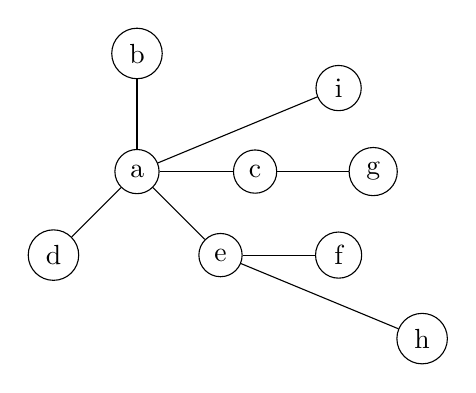
\begin{tikzpicture}[node distance=15mm, main/.style = {draw, circle}] 
        \node[main] (A) {a}; 
        \node[main] (B) [above of=A] {b}; 
        \node[main] (C) [right of=A] {c}; 
        \node[main] (D) [below left of=A] {d}; 
        \node[main] (E) [below right of=A] {e}; 
        \node[main] (F) [right of=E] {f}; 
        \node[main] (G) [right of=C] {g}; 
        \node[main] (H) [below right of=F] {h}; 
        \node[main] (I) [above right of=C] {i}; 
        
        \draw (A) -- (B); 
        \draw (A) -- (C); 
        \draw (A) -- (D); 
        \draw (A) -- (I); 
        \draw (A) -- (E); 
        
        \draw (C) -- (G); 
        \draw (E) -- (F); 
        \draw (E) -- (H); 
    \end{tikzpicture}

    \vspace{0.5cm}
    \textbf{Complexity Analysis:}
    \begin{itemize}
        \item Sorting edges takes \( O(E \log E) \).
        \item Each Union-Find operation runs in \( O(\log V) \).
        \item Overall time complexity: \( O(E \log E + E \log V) = \theta(E \log V) \).
        \item Efficient for sparse graphs where \( E \approx O(V) \).
    \end{itemize}
\end{frame}



\begin{frame}{Prim’s Algorithm for MST}
    \textbf{Step 1:} Start with an arbitrary vertex (e.g., \( V[0] \)). \\
    \textbf{Step 2:} Pick the smallest outgoing edge that connects to an unvisited vertex. \\
    \textbf{Step 3:} Add this edge to the Minimum Spanning Tree (MST). \\
    \textbf{Step 4:} Repeat until all vertices are included in the MST. \\
\end{frame}

% Frame 1: Original Graph
\begin{frame}{Graph Representation}
    \centering
    \begin{tikzpicture}[node distance=15mm, main/.style = {draw, circle}] 
        % Nodes
        \node[main] (A) {a}; 
        \node[main] (B) [right=of A] {b}; 
        \node[main] (C) [below left=of A] {c}; 
        \node[main] (D) [below=of A] {d}; 
        \node[main] (E) [below=of B] {e}; 
        \node[main] (F) [right=of B] {f}; 
        \node[main] (G) [below left=of D] {g}; 
        \node[main] (H) [below=of E] {h}; 

        % Edges with weights
        \draw[-] (A) -- (B) node[midway, above] {3}; 
        \draw[-] (A) -- (C) node[midway, left] {2}; 
        \draw[-] (B) -- (F) node[midway, above] {7}; 
        \draw[-] (B) -- (E) node[midway, right] {19}; 
        \draw[-] (A) -- (D) node[midway, right] {0}; 
        \draw[-] (C) -- (G) node[midway, left] {1}; 
        \draw[-] (D) -- (E) node[midway, above] {-4}; 
        \draw[-] (D) -- (G) node[midway, left] {1}; 
        \draw[-] (D) -- (H) node[midway, left] {-2}; 
        \draw[-] (G) -- (H) node[midway, below] {9}; 
        \draw[-] (E) -- (H) node[midway, right] {5}; 
        \draw[-] (F) -- (H) node[midway, right] {6}; 
    \end{tikzpicture}
\end{frame}

% Frame 2: Prim's Algorithm - Minimum Spanning Tree
\begin{frame}{Prim's Algorithm - Minimum Spanning Tree}
    \centering
    \begin{tikzpicture}[node distance=15mm, main/.style = {draw, circle}] 
        % Nodes
        \node[main] (A) {a}; 
        \node[main] (B) [right=of A] {b}; 
        \node[main] (C) [below left=of A] {c}; 
        \node[main] (D) [below=of A] {d}; 
        \node[main] (E) [below=of B] {e}; 
        \node[main] (F) [right=of B] {f}; 
        \node[main] (G) [below left=of D] {g}; 
        \node[main] (H) [below=of E] {h}; 

        % Highlighted MST edges (Correct Prim's Algorithm)
        \draw[red, very thick] (D) -- (E) node[midway, above] {-4}; 
        \draw[red, very thick] (D) -- (A) node[midway, right] {0}; 
        \draw[red, very thick] (D) -- (G) node[midway, left] {1}; 
        \draw[red, very thick] (G) -- (C) node[midway, left] {1}; 
        \draw[red, very thick] (A) -- (B) node[midway, above] {3}; 
        \draw[red, very thick] (D) -- (H) node[midway, right] {-2}; 
        \draw[red, very thick] (H) -- (F) node[midway, right] {6}; 

        % Non-MST edges (Faded)
        \draw[gray, dashed] (B) -- (F) node[midway, above] {7}; 
        \draw[gray, dashed] (B) -- (E) node[midway, right] {19}; 
        \draw[gray, dashed] (C) -- (A) node[midway, left] {2}; 
        \draw[gray, dashed] (E) -- (H) node[midway, left] {5}; 
        \draw[gray, dashed] (G) -- (H) node[midway, below] {9}; 
    \end{tikzpicture}
\end{frame}

\begin{frame}{Prim's Algorithm - Path Explanation}
    \textbf{Path Taken:}
    \begin{itemize}
        \item Start at node \( D \), selecting the edge \( D \to E \) with the minimum weight \(-4\).
        \item Select \( D \to H \) (cost \( -2 \)) as the next smallest edge.
        \item Pick \( D \to A \) (cost \( 0 \)), the next lowest cost edge.
        \item Choose \( D \to G \) (cost \( 1 \)) to expand the MST.
        \item Select \( G \to C \) (cost \( 1 \)), as it connects a new node with minimal cost.
        \item Add \( A \to B \) (cost \( 3 \)), as it’s the cheapest edge connecting a new node.
        \item Finally, add \( H \to F \) (cost \( 6 \)), completing the MST.
    \end{itemize}
\end{frame}



\begin{frame}{Efficiency of Prim’s Algorithm}
    \begin{itemize}
        \item Uses a \textbf{priority queue} (typically a min-heap).
        \item Extracting the minimum edge takes \( O(\log E) \).
        \item Processing all edges results in \( O(E \log E) \).
        \item Overall complexity: \( \theta(E \log E) \).
    \end{itemize}
\end{frame}

\begin{frame}{Graph Algorithms Overview}
    \textbf{1. Topological Sorting (DAG Only)}
    \begin{itemize}
        \item Orders vertices such that for every edge $(u, v)$, $u$ appears before $v$.
        \item \textbf{Kahn’s Algorithm (BFS):} Uses in-degree and a queue.
        \item \textbf{DFS-Based}: Uses a stack for reverse order.
    \end{itemize}

    \textbf{2. Minimum Spanning Tree (MST)}
    \begin{itemize}
        \item Connects all vertices with the **minimum total edge weight**.
        \item Two main algorithms:
        \begin{itemize}
            \item \textbf{Kruskal’s (Edge-based, uses Union-Find).}
            \item \textbf{Prim’s (Vertex-based, uses Priority Queue).}
        \end{itemize}
    \end{itemize}
\end{frame}

\begin{frame}{Kruskal’s, Prim’s, and Union-Find}
    \textbf{3. Kruskal’s Algorithm (Greedy)}
    \begin{itemize}
        \item Sorts edges by weight and adds the smallest edge without forming a cycle.
        \item Uses \textbf{Union-Find} to track connected components.
    \end{itemize}

    \textbf{4. Union-Find (Disjoint Set)}
    \begin{itemize}
        \item \textbf{Find(x)}: Finds the root of the set.
        \item \textbf{Union(x, y)}: Merges sets using **path compression**.
    \end{itemize}

    \textbf{5. Prim’s Algorithm (Greedy)}
    \begin{itemize}
        \item Starts from any vertex, picks the smallest edge using a **min-heap**.
        \item Grows the MST by adding one vertex at a time.
    \end{itemize}

    \textbf{Comparison:}
    \begin{itemize}
        \item \textbf{Prim’s:} Better for **dense** graphs.
        \item \textbf{Kruskal’s:} Better for **sparse** graphs.
    \end{itemize}
\end{frame}






